% ============================================================================
% Two_Breaks — ApJ draft, written in the Li et al. (2021, ApJS 254,35) style.
% FILLED with PROVISIONAL numbers from the clean re-fit (results/clean_per_burst/,
% corrected backgrounds + clean blocks + multi-start BB engine; results computed by
% scripts/31_draft_numbers.py -> results/draft_numbers.json).  These numbers will
% be FINALISED after Khushboo's human background verification -> re-fit; the
% qualitative conclusions are not expected to change.  Model descriptions follow
% Ravasio et al. (2SBPL) + Guiriec et al. (multi-component).  %chk before submit.
% ============================================================================
\documentclass[twocolumn]{aastex631}

\newcommand{\nuc}{\ensuremath{\nu_c}}
\newcommand{\num}{\ensuremath{\nu_m}}
\newcommand{\Ep}{\ensuremath{E_{\rm p}}}
\newcommand{\kT}{\ensuremath{kT}}
\newcommand{\Liso}{\ensuremath{L_{\rm iso}}}
\newcommand{\daic}{\ensuremath{\Delta\mathrm{AIC}}}
\newcommand{\ssc}{\ensuremath{\sigma_{\rm sc}}}
% residual placeholder macros (should no longer appear in the body):
\newcommand{\PH}[1]{\ensuremath{\mathbf{[#1]}}}
\newcommand{\PHt}[1]{\textbf{[#1]}}
% figure placeholder box (real data figures at Phase 5):
\newcommand{\figph}[2][0.26\textheight]{\fbox{\parbox[c][#1][c]{0.92\linewidth}{%
  \centering\itshape Figure placeholder.\\ #2}}}

\shorttitle{Empirical Time-Resolved Spectroscopy of Single-Pulse GRBs}
\shortauthors{Sharma et al.}

\begin{document}

\title{Time-Resolved Empirical Spectroscopy of a Large Sample of Single-Pulse
Gamma-Ray Bursts: Thermal versus Two-Break Origins of the Spectral Curvature}

% %TODO author names/affiliations/ORCIDs are placeholders.
\author{Khushboo Sharma}
\affiliation{Affiliation TBD}
\author{B}
\affiliation{Affiliation TBD}
\email{vikas.chand.physics@gmail.com}
\author{C}
\affiliation{Affiliation TBD}

\begin{abstract}
Gamma-ray bursts (GRBs) are highly variable and exhibit strong spectral
evolution, and the physical origin of their prompt emission remains debated.
Here we present a time-resolved spectral analysis of a uniform sample of
$106$ single-pulse, bright Fermi/GBM bursts, comprising $1057$
time-resolved spectra, fit with a family of empirical photon models---the Band
function, a cutoff power law, a smoothly broken power law, a double smoothly
broken power law (2SBPL), and the two non-thermal continua each with an added
blackbody. We use empirical models as a model-agnostic probe and ask whether the
thermal--non-thermal $\Ep$--$\kT$ correlation reported by \citet{Burgess2014a}
for six bursts appears in a large sample, and what additional spectral properties
emerge. We find that the low-energy photon index peaks at $\alpha\approx-0.7$,
between the slow- and fast-cooled synchrotron limits ($-2/3$ and $-3/2$); that
$91\%$ ($151/166$) of the time bins requiring curvature beyond a single break are
equally or better described by adding a blackbody than by an explicit
second break (the $9\%$ two-break fraction is a lower limit); and that where a
blackbody is decisively required ($\Delta\mathrm{AIC}\ge10$), the
\citet{Burgess2014a} correlation is recovered in $89\%$ ($17/19$) of testable
bursts, most strikingly in GRB~130427A ($\rho=0.93$, $\Ep\propto\kT^{0.9}$).
We further find a positive correlation between the two synchrotron break
energies ($\rho=0.57$; intrinsic scatter $0.38$~dex), present both within and
between bursts. We caution, however, that no single empirical model is decisively
preferred over the next-best alternative in $92\%$ ($875/950$) of comparable
bins, and that an empirical continuum can absorb a sub-dominant thermal
component. We discuss the implications for the prompt radiation mechanism and
jet composition.
\end{abstract}

\keywords{Gamma-ray bursts (629) --- Spectroscopy (1558) --- Non-thermal
radiation sources (1119) --- Astrostatistics (1882)}

% ============================================================================
\section{Introduction} \label{sec:intro}
% ============================================================================
Gamma-ray bursts (GRBs) are highly variable and exhibit strong spectral
evolution, with the $\nu F_\nu$ peak energy \Ep\ and the low-energy photon index
$\alpha$ typically varying with the prompt light curve
\citep[e.g.,][]{Norris1996,Kaneko2006,Lu2012,Yu2016}. To first order the prompt
spectrum is well described by the empirical Band function \citep{Band1993} or a
cutoff power law, yet these functions are physically agnostic: the same curvature
can arise from distinct emission mechanisms, and the fitted parameters do not by
themselves identify the radiative process \citep[e.g.,][]{KumarZhang2015}.

Two physically motivated pictures dominate. In the first, part of the prompt flux
is quasi-thermal emission from the jet photosphere, approximated by a blackbody
(BB) superposed on a non-thermal continuum
\citep[e.g.,][]{MeszarosRees2000,Ryde2004,Peer2007,Guiriec2010,Guiriec2011}.
Fitting a physical synchrotron-plus-blackbody model to six bright single-pulse
bursts, \citet{Burgess2014a} reported a tight per-burst correlation
$\Ep\propto\kT^{\alpha}$, interpreting $\alpha\!\sim\!1$ as a baryon-dominated
and $\alpha\!\sim\!2$ as a magnetically-dominated jet. In the second picture, the
curvature is optically-thin synchrotron radiation from a cooling electron
population, which imprints \emph{two} characteristic break energies: the cooling
frequency \nuc\ and the injection frequency \num\ \citep{Sari1998}. A double
smoothly broken power law (2SBPL) captures both breaks and has been used to argue
for a synchrotron origin
\citep[e.g.,][]{Oganesyan2017,Oganesyan2018,Ravasio2018,Ravasio2019}. Most
recently, \citet{Mei2025} found that, under the synchrotron interpretation, the
fundamental spectral--energetics relation is between \nuc\ and the isotropic
luminosity rather than the classical $\Ep$--\Liso\ relation
\citep[the Yonetoku relation;][]{Yonetoku2004}.

Crucially, the two pictures produce similar curvature near the spectral peak: a
blackbody on a single-break continuum (BB$+$SBPL) is an effective \emph{proxy}
for a 2SBPL. Distinguishing them, and characterizing the resulting spectral
properties at scale, is the goal of this work. Single-pulse bursts offer the
cleanest test, since a single, non-overlapping pulse exhibits the simplest
spectral evolution and avoids the blending of distinct emission episodes
\citep[e.g.,][]{RydePeer2009,Basak2014,Burgess2014b,Busby2024}.
\citet{Basak2014} performed exactly such a time-resolved study of nine
single-pulse Fermi bursts with thermal-family models, finding that a blackbody
peaks well below the Band $\nu F_\nu$ peak and that $\alpha$ frequently exceeds
the synchrotron limit, especially in hard-to-soft pulses; \citet{Burgess2014a}
were limited to six bursts. Whether these results are general has not been tested
on a large, uniformly-analyzed sample.

In this paper we take a deliberately empirical approach. We fit a family of
model-agnostic functions uniformly to a large, single-pulse sample, and we
investigate (i) the distributions and time evolution of the spectral parameters,
(ii) the correlations among them, (iii) whether the \citet{Burgess2014a}
$\Ep$--$\kT$ correlation appears in a large sample, and (iv) what additional
spectral properties---in particular a relation between the two synchrotron
breaks---emerge. The paper is organized as follows. Section~\ref{sec:method}
describes the sample, data reduction, and spectral fitting; Section~\ref{sec:obs}
presents the observed parameter distributions, spectral evolution, and
correlations; Section~\ref{sec:emission} assesses the compatibility with emission
models; Section~\ref{sec:discussion} discusses the results; and
Section~\ref{sec:summary} summarizes our findings. Uncertainties are quoted at the
1$\sigma$ (68\%) level unless stated otherwise.

% ============================================================================
\section{Methodology} \label{sec:method}
% ============================================================================
\subsection{Initial Burst Selection} \label{sec:sel}
We select single-pulse bursts from the Fermi/GBM catalog
\citep{Meegan2009,Gruber2014} using the shape-based ``horizontal-line'' algorithm
of \citet{Busby2024}, which scores how well a single FRED-like pulse describes the
background-subtracted light curve. We retain bursts above the \citeauthor{Busby2024}
single-pulse threshold (score $\gtrsim0.9983$) and apply a fluence cut of
$>$$10^{-5}$~erg~cm$^{-2}$ (10--1000~keV, GBM catalog) to ensure adequate
time-resolved signal-to-noise, since a robust spectral shape requires
sufficient counts per bin (Section~\ref{sec:bin}). No $T_{90}$ restriction is
imposed; the sample therefore contains both short- and long-duration bursts whose
emission is dominated by a single pulse. We emphasize that this selection is on
pulse \emph{shape}, not brightness: the sample fluence spans a factor of
$\sim$$250$. The final sample comprises \textbf{$106$} bursts
(Table~\ref{tab:sample}).

\subsection{Detector, Source, and Background Selections} \label{sec:bkg}
For each burst we use the time-tagged event (TTE) data of the NaI detectors
within $\sim50^\circ$ (relaxed to $60^\circ$ where required to retain a
triggering detector) of the source, the most-illuminated BGO, and, for the
$11$ bursts with usable LAT Low-Energy (LLE) data (a subset of the $18$
LAT-detected bursts), the LLE data above 30~MeV \citep{Atwood2009}, with the
corresponding response matrices; for multi-epoch \texttt{rsp2} responses the
matrix covering the source interval is used. We use 8--900~keV for NaI (the
33--40~keV iodine K-edge region masked; \citealt{Ronchi2020}), 0.3--40~MeV for
BGO, and 30--100~MeV for LLE. Inter-detector calibration is handled by free
effective-area constants in the range 0.8--1.2, frozen to unity for the
reference NaI \citep[as in][]{Ronchi2020}. The source interval is set to bracket the burst emission,
and two background intervals (pre- and post-burst) are fit
with a time polynomial of order $\le$3, the order chosen by a likelihood-ratio
test, and interpolated beneath the burst. Background windows are selected by an
automated peak-centered algorithm: the emission interval is located from the
cumulative background-subtracted counts, the source window brackets it, and
pre/post background windows of up to 80~s (40~s minimum on the wider side,
asymmetric for bursts that peak early in the data span) are placed on either
side and validated against the light curve; an accurate background is the
prerequisite for recovering any sub-dominant spectral component. Independent
human verification of every window, targeting 50--150~s background intervals
per detector, is in progress and will supersede the automated
catalog.\footnote{The numbers in this paper therefore use the provisional,
automatically-selected background catalog; the qualitative conclusions are not
expected to be sensitive to this refinement.}

\subsection{Light-curve Binning} \label{sec:bin}
We define the time bins with the Bayesian Blocks algorithm \citep{Scargle2013}
in its binned (count-rate) mode, applied to the 8--900~keV light curve of a
reference NaI detector (the first GBM-catalog--selected NaI) at 0.128~s
resolution with a false-alarm probability $p_0=0.01$ (for two over-coarse
bursts, 0.064~s and $p_0=0.05$), and we map the resulting change points to all
detectors. The source window is first tightened to the emission interval, and
leading/trailing blocks with net significance below $4.5\sigma$ are trimmed.
This minimizes intra-bin spectral evolution while preserving signal. Each block
is one spectral fit; the procedure yields \textbf{$1057$} time-resolved spectra.

\subsection{Block Definition and Grading} \label{sec:grade}
We grade each burst by the quality of its time-resolved coverage, following a
three-tier scheme:
\begin{enumerate}
\item \emph{Gold}: $40$ bursts with $\ge10$ well-constrained
  bins, suitable for per-burst parameter relations.
\item \emph{Silver}: $44$ bursts with $5$--$9$ bins, contributing to
  population statistics with caveats.
\item \emph{Bronze}: $22$ bursts with $\le4$ bins, too few for per-burst
  trends; included only in the pooled distributions.
\end{enumerate}
The grade is carried as a column in Table~\ref{tab:perburst} and is used in
Section~\ref{sec:discussion} to show that our main results hold on the cleanest
(Gold) subsample.

\subsection{Spectral Models} \label{sec:models}
We fit each spectrum with six photon models spanning the two interpretations of
the spectral curvature while remaining empirical and comparable with the GBM
catalogs \citep[e.g.,][]{Kaneko2006,Gruber2014}. Empirical functions are flexible
and model-agnostic; although they do not map uniquely onto a mechanism, the
low-energy index $\alpha$ still discriminates between scenarios at high
significance \citep[e.g.,][]{Acuner2020}.

The Band function \citep{Band1993} is a smoothly-joined broken power law; below
the break $E_b=(\alpha-\beta)\Ep/(2+\alpha)$,
\begin{equation}
N(E)=A\,(E/E_0)^{\alpha}\,\exp\!\left[-(2+\alpha)E/\Ep\right],
\end{equation}
joining $N(E)\propto E^{\beta}$ above $E_b$, with $E_0=100$~keV. The cutoff power
law (CPL), $N(E)=A\,(E/E_0)^{\Gamma}\exp(-E/E_c)$ with $\Ep=(2+\Gamma)E_c$, is the
$\beta\!\to\!-\infty$ limit. The smoothly broken power law (SBPL) joins two
power-law segments with photon indices $\alpha$ and $\beta$ at a break energy
$E_{\rm b}$, with the sharpness of the join an adjustable parameter; we use
the GBM-catalog parameterization \citep{Kaneko2006} as implemented in
\textsf{astromodels}, with the break scale held fixed.

To represent the synchrotron interpretation we use the double smoothly broken
power law \citep[2SBPL;][whose Equations~1--4 give the functional
form]{Ravasio2018}: three power-law segments with photon indices
$\alpha_1,\alpha_2,\beta$ joined at two break energies---a lower break $x_b$
and an upper break $x_p$ (the latter at the $\nu F_\nu$ peak)---each join
having a sharpness parameter ($n_1$, $n_2$). We fit the
\textsf{astromodels} implementation, whose free parameters are the
normalization, the three indices, and the two break energies. Under the
optically-thin synchrotron interpretation the two breaks are
physical---$x_b$ is the cooling frequency \nuc\ and $x_p=\num$ the injection
frequency---and the segment between them carries the synchrotron slopes
$\alpha_1\simeq-2/3$ (slow cooling) steepening toward $-3/2$ (fast cooling)
\citep[e.g.,][]{Sari1998,Ravasio2019}. We hold the break sharpnesses fixed
($n_1=n_2=2$ in this provisional run; the verified re-fit will adopt the
$n_1=5.38$, $n_2=2.69$ calibration of \citealt{Ravasio2018}, who found that
leaving $n_1$ free does not converge reliably---the same behavior we observe).
The full fit configuration (parameter bounds, seeds, and restart grids) is
listed in Appendix~\ref{app:fitconfig}.

To represent the photospheric interpretation we add a blackbody to the two
simplest non-thermal continua, following the multi-component decomposition of
\citet{Guiriec2011,Guiriec2015}, in which a sub-dominant quasi-thermal component
accompanies the non-thermal emission and the two are fit \emph{simultaneously}.
The blackbody photon spectrum is $N(E)\propto E^{2}/[\exp(E/\kT)-1]$, and we form
the composites Band$+$BB and CPL$+$BB; we quantify the thermal contribution by the
flux ratio $F_{\rm BB}/F_{\rm tot}$ \citep{Guiriec2015}. A BB$+$SBPL composite
reproduces the curvature of a 2SBPL near the peak, so the $+$BB models act as a
practical thermal proxy for the two-break model.

\subsection{Spectral Fitting and Model Selection} \label{sec:fit}
All fits are performed in the Multi-Mission Maximum Likelihood framework
\citep[3ML;][]{Vianello2015} with the \texttt{pgstat} likelihood (a Poisson
source with Gaussian background). Model comparison uses the Akaike and Bayesian
information criteria \citep[AIC, BIC;][]{Akaike1974,Schwarz1978} computed from
the standard $-2\ln L$, applied according to the relationship between the models
compared. For \emph{nested} pairs (Band$+$BB/Band, CPL$+$BB/CPL, 2SBPL/SBPL) a
blackbody or second break is deemed significant at $\daic\ge10$ relative to the
parent continuum---the AIC analog of the $\Delta\mathrm{DIC}\ge10$ threshold of
\citet{Li2021} and the Bayes-factor threshold ($2\ln K>10$) of
\citet{Burgess2019}, and equivalent here to a likelihood-ratio statistic
\citep{Wilks1938} of $\ge$$14$, beyond the nominal 99\% (2~d.o.f.) point; we
prefer the information-criterion form because the $\chi^2$ calibration of the
classical LRT is only approximate when a component normalization sits at a
parameter boundary. Every blackbody and second break that passes $\daic\ge10$
also passes the more conservative $\Delta\mathrm{BIC}$ criterion. For
\emph{non-nested} comparisons---in particular the central thermal
($+$BB) versus two-break (2SBPL) question---the LRT is inapplicable and we rely
on \daic\ alone, with $\Delta\mathrm{BIC}$ as a cross-check. A physical-validity
gate prevents a fit from \emph{winning} the selection if any key parameter is
railed against a bound or, for the 2SBPL, if the breaks are mis-ordered
($x_b\ge x_p$); in the $4\%$ ($43/1057$) of bins where no model passes the gate
we assign no preferred model. The blackbody possesses a railing local minimum,
so we multi-start the $+$BB models whose blackbody is railed or insignificant
from a grid of temperature seeds and retain the lowest $-2\ln L$. The 2SBPL has
no analogous restart in the present (provisional) run, so two-break counts are
conservative lower limits (Section~\ref{sec:curv}). We quantify each parameter
correlation by the Spearman rank coefficient $\rho$ and a least-squares slope in
log space. Energy and photon fluxes are obtained by integrating the best-fit
Band model over 10--1000~keV, with uncertainties propagated by Monte Carlo over
the fitted parameter uncertainties (200 draws; 16th--84th percentiles). For the
principal $\num$--$\nuc$ relation, whose two variables carry comparable
uncertainties, we maximize the \citet{DAgostini2005} errors-in-both-variables
likelihood,
\begin{equation}
-2\ln\mathcal{L}=\sum_i\left[\ln 2\pi\sigma_i^2
+\frac{(y_i-m x_i-c)^2}{\sigma_i^2}\right],\quad
\sigma_i^2=\ssc^2+\sigma_{y,i}^2+m^2\sigma_{x,i}^2,
\label{eq:dagostini}
\end{equation}
with the measured break uncertainties (in dex) on both axes and the intrinsic
scatter \ssc\ a free parameter.

% ============================================================================
\section{Observational Properties} \label{sec:obs}
% ============================================================================
Throughout this section, each statistic is computed on the subset of the
$1057$ bins for which the relevant quantity is constrained: $792$ bins
($75\%$) have a physically valid Band fit (the reference for $\alpha$, \Ep,
and flux); $301$ bins have a decisive blackbody ($\daic\ge10$;
Section~\ref{sec:fit}), of which $233$ also have a valid Band flux; $349$ bins
have a valid 2SBPL with ordered breaks; $950$ bins have at least two
physically valid models (the model-comparison set); and per-burst statistics
use the $100$ bursts with at least one valid Band bin, with per-burst
correlations requiring $\ge$$5$ bins ($68$ bursts) or $\ge$$4$
$\Ep$--$\kT$ pairs ($19$ bursts).

\subsection{Parameter Distributions} \label{sec:dist}
We now examine the distributions of the spectral parameters
(Figure~\ref{fig:dist}, Table~\ref{tab:dist}). The low-energy index has a
median $\alpha=-0.71\pm0.49$, the peak energy $\log_{10}(\Ep/{\rm keV})=
2.28\pm0.40$ (median $\Ep\simeq192$~keV), and the high-energy index a median
$\beta=-2.6$, in agreement with previous catalogs
\citep[e.g.,][]{Kaneko2006,Gruber2014}. The blackbody temperature, where
decisively required, has a median $\kT\simeq28$~keV and spans
$\kT\approx3$--$70$~keV (5th--95th percentiles), bracketing the
$\sim$$40$~keV temperatures of \citet{Guiriec2015}. K-S tests between tiers
(Table~\ref{tab:ks}) show that the Gold-tier distributions differ modestly from
the lower tiers ($p\approx0.004$ for $\alpha$, $0.03$ for $\log\Ep$), as
expected since the brightest bursts populate the Gold tier; the difference does
not affect the conclusions below.

\begin{figure*}[t]
\centering
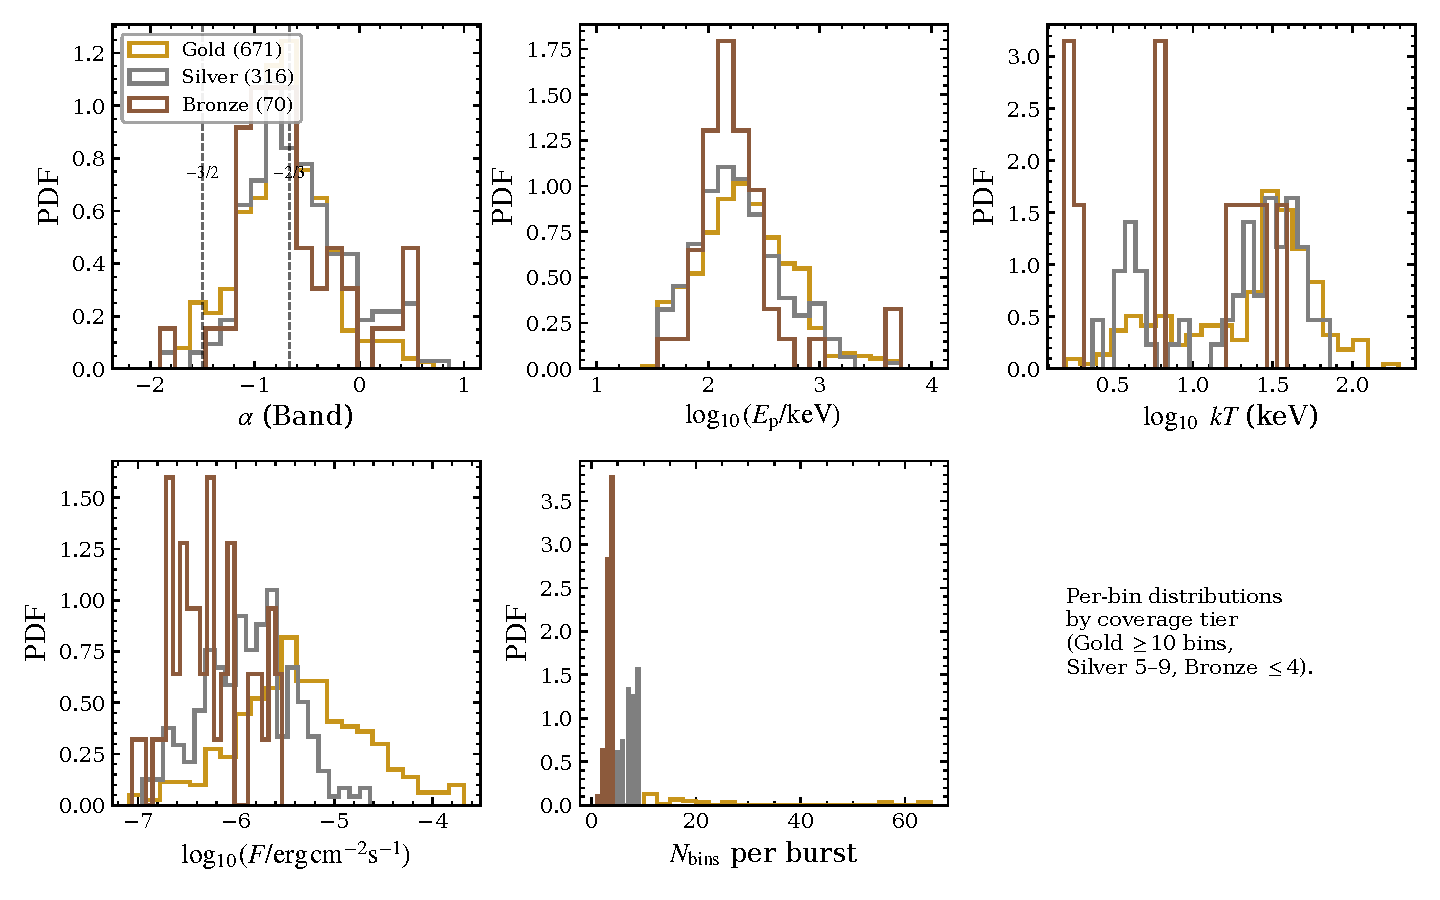
\includegraphics[width=0.95\textwidth]{two_break_figures/fig_dist.pdf}
\caption{Distributions of the Band low-energy index $\alpha$, peak energy \Ep,
blackbody temperature \kT, energy flux $F$, and the number of bins per burst,
split by coverage tier (Gold/Silver/Bronze). The legend gives the total number
of time bins per tier ($1057$ in all); each panel shows the subset in which the
plotted parameter is constrained. Dashed lines in the $\alpha$ panel mark the
slow- and fast-cooled synchrotron limits ($-2/3$, $-3/2$).}
\label{fig:dist}
\end{figure*}

\subsection{Spectral Evolution} \label{sec:evol}
We classify the \Ep\ evolution into hard-to-soft (HTS) and intensity-tracking
(IT) patterns following the physical discriminant of \citet{Lu2012} and
\citet{Basak2014}: the two classes differ in the \emph{rising} phase of the
pulse, where an IT pulse hardens with the flux while an HTS pulse is already at
its hardest and softening (in the decay phase both soften together, so a
whole-pulse $\Ep$--flux correlation cannot separate them). We therefore
classify on the pre-peak behavior---the sign of the $\Ep$ trend through the
flux peak, falling back to the position of the \Ep\ maximum when the rise is
covered by fewer than three bins. Of the $76$ bursts with $\ge$$4$ classifiable
bins, $63\%$ ($48/76$) are HTS, $25\%$ ($19/76$) are IT, and $12\%$ ($9/76$)
are ambiguous (Figure~\ref{fig:evol}), an HTS-dominated mix consistent with the
small single-pulse samples of \citet{Lu2012} and \citet{Basak2014}. The general
trend is that pulses soften over time, with $\alpha$ decreasing through the
pulse.

\begin{figure*}[t]
\centering
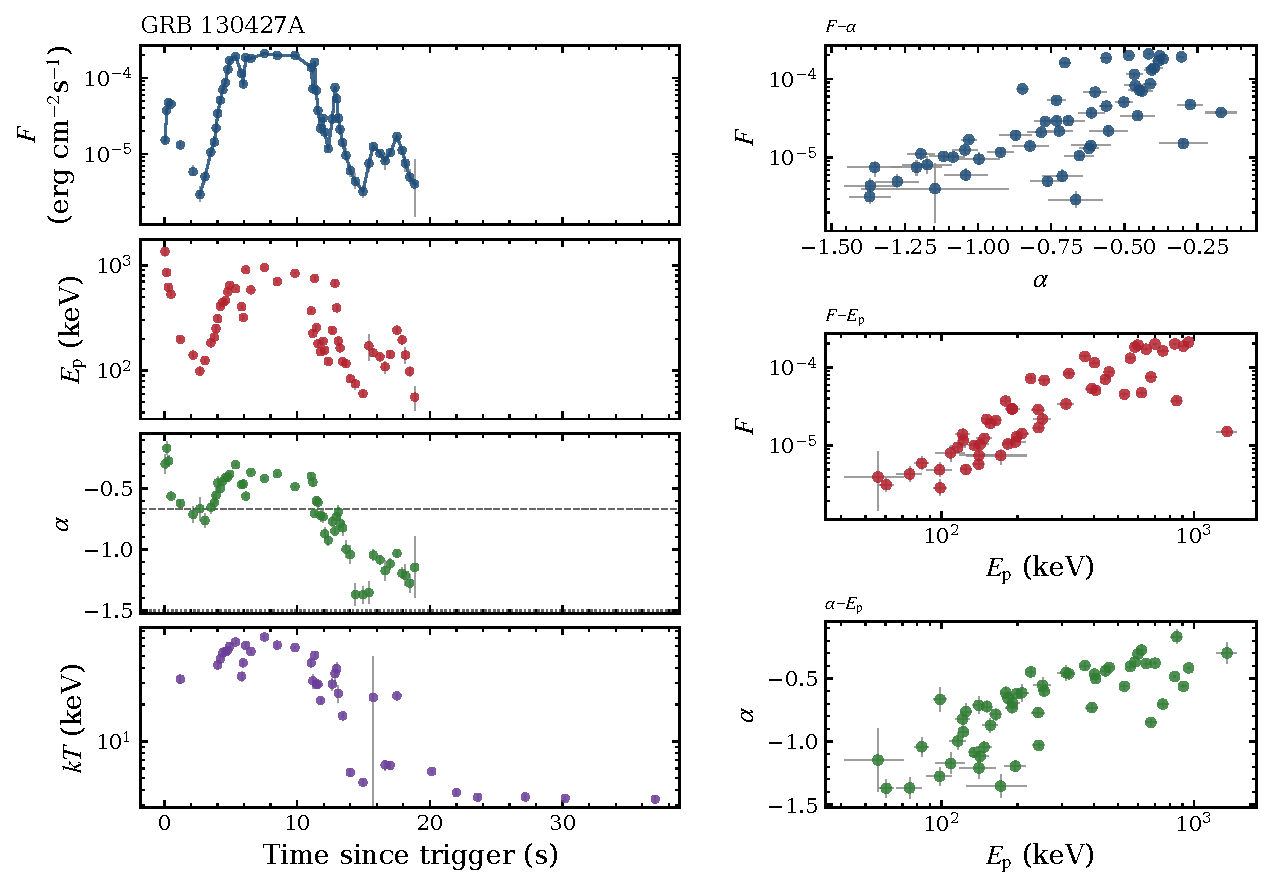
\includegraphics[width=\textwidth]{two_break_figures/fig_evol.pdf}
\caption{Time-resolved spectral evolution of GRB~130427A ($65$ bins in all).
Left, top to bottom: the energy-flux light curve $F(t)$, $\Ep(t)$, $\alpha(t)$
(dashed/dotted lines at $-2/3$, $-3/2$), and $\kT(t)$. Each panel shows the
bins in which the plotted quantity is constrained ($54$ Band-valid bins for
$F$, \Ep, $\alpha$; decisive-blackbody bins for $\kT$, which extend into the
late tail). Right: the $F$--$\alpha$, $F$--$\Ep$, and $\alpha$--$\Ep$ relations
for the same burst.}
\label{fig:evol}
\end{figure*}

\subsection{Parameter Correlations} \label{sec:corr}
Turning to the parameter correlations, we fit each pair with the functional forms
adopted by \citet{Li2021} and report both the per-burst incidence and the pooled,
sample-wide trend (Table~\ref{tab:curv}).

\subsubsection{The $F$--$\alpha$ Relation}
We fit $F=F_0\,e^{k\alpha}$ and find a positive correlation in $84\%$ ($57/68$)
of bursts, with pooled $k=0.27$: brighter spectra tend to have harder low-energy
indices, though the trend is weak (pooled $\rho=0.17$).

\subsubsection{The $F$--$\Ep$ Relation}
We fit a power law $F\propto\Ep^{\,k_1}$ and find $k_1=0.66$, positive in $94\%$
($64/68$) of bursts (pooled $\rho=0.43$). This correlation, however, is partly
\emph{induced}: an empirical model's energy flux and \Ep\ are not independent. In
photon flux the rank correlation collapses to $\rho=0.15$, consistent with the
absence of an intrinsic $\Ep$--luminosity relation \citep{Mei2025}.

\subsubsection{The $\alpha$--$\Ep$ Relation}
We fit $\alpha=k_2\log_{10}\Ep+c$ and find only a weak positive trend,
$k_2=0.02$ (pooled $\rho=0.10$); a positive per-burst correlation appears in
$66\%$ ($45/68$) of bursts but is individually significant in only a handful.

\subsection{Curvature and the Two Pictures} \label{sec:curv}
We now turn to the curvature beyond a single spectral break, the central question
of this work. Restricting to bins requiring such curvature ($\daic>6$ relative to
the best single-break model, with the curved model physically valid), we classify
each as thermal ($+$BB preferred) or two-break (2SBPL preferred with
$\daic\ge10$ over the SBPL); the remainder are degenerate between the two
pictures (Table~\ref{tab:curvsplit}). Of the $166$ such bins, $91\%$
($151/166$) are thermal-or-degenerate and $9\%$ ($15/166$) decisively prefer
the explicit second break ($87\%$/$13\%$ at the stricter $\daic\ge10$
curvature cut); because the 2SBPL carries no convergence restart in this run
(Section~\ref{sec:fit}), the two-break fractions are lower limits. More
broadly, no single empirical model is decisively preferred over the next-best
alternative ($\daic<10$) in $92\%$ ($875/950$) of the bins with at least two
valid models---and all valid models agree within $\daic<10$ in $58\%$---echoing
the difficulty \citet{Basak2014} noted in separating thermal and non-thermal
descriptions on goodness-of-fit alone. Where a blackbody is decisively
required, its flux fraction is typically small but spans a wide range
($F_{\rm BB}/F_{\rm tot}$ median $0.006$, interquartile $0.001$--$0.10$): the
brightest bins permit detection of percent-level blackbodies, so the median
reflects detectability as much as physics, with the upper quartile matching the
$1$--$10\%$ energy fractions of \citet{Guiriec2015}. Testing the
\citet{Burgess2014a} relation per burst on the decisive-blackbody sample, the
$\Ep$--$\kT$ correlation is positive in $89\%$ ($17/19$) of testable bursts
($12$ individually significant), most cleanly in the highest signal-to-noise
bursts (GRB~130427A: $\rho=0.93$, $\Ep\propto\kT^{0.88\pm0.07}$;
GRB~160625B: $\rho=0.78$); fainter bursts yield too few decisive-blackbody bins
to test, a consequence of the empirical continuum absorbing the thermal
curvature. Finally, the two 2SBPL breaks are positively correlated
($\rho=0.57$, $N=349$): the \citet{DAgostini2005} fit gives
$\num\propto\nuc^{\,0.46\pm0.05}$ with intrinsic scatter \ssc$=0.38$~dex, and,
unlike a pure inter-burst artifact, the relation is significant both within
($\rho=0.43$) and between ($\rho=0.51$) bursts (Section~\ref{sec:disc-breaks}).

\begin{figure*}[t]
\centering
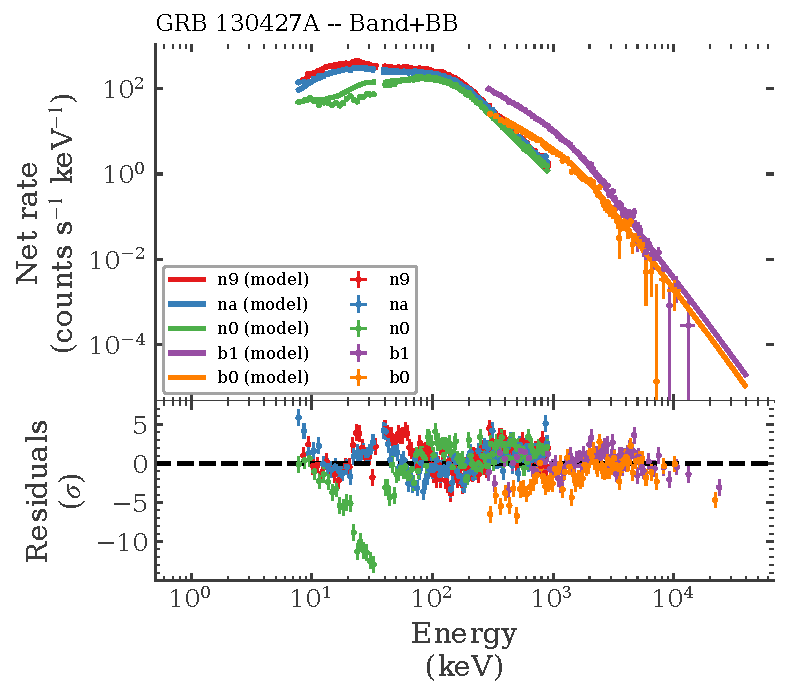
\includegraphics[width=0.46\textwidth]{two_break_figures/fig_spec_a.pdf}\hfill
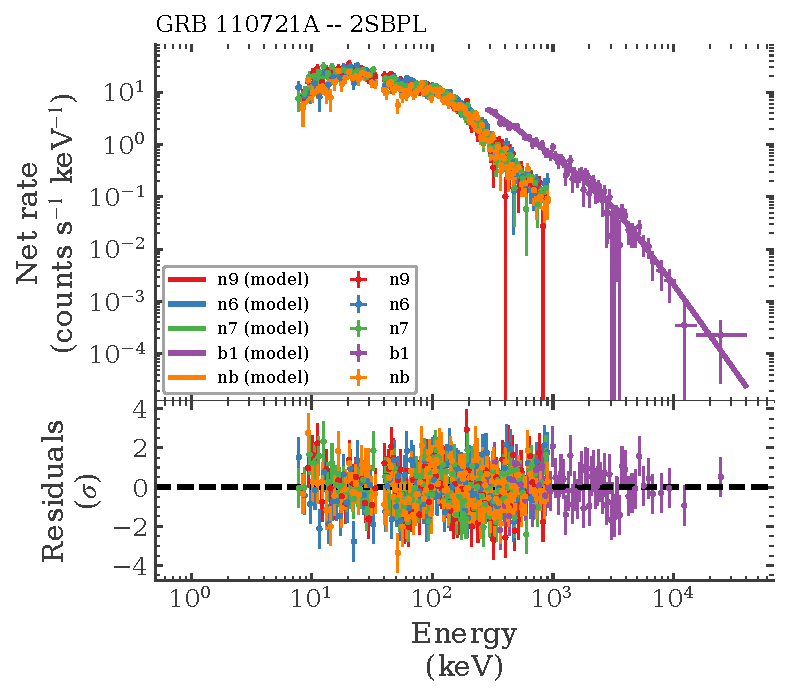
\includegraphics[width=0.46\textwidth]{two_break_figures/fig_spec_b.pdf}
\caption{Count spectra and residuals for the two emblematic curvature cases.
Left: a decisively blackbody-requiring bin of GRB~130427A ($8.7$--$11.0$~s)
fit with Band$+$BB, chosen away from the flux peak where pile-up may affect
this exceptionally bright burst \citep[cf.][]{Mei2025}; the narrow low-energy
residual structure in one NaI is of the kind attributed to response
calibration and intra-bin spectral evolution in very bright bursts
\citep[cf.][]{Ronchi2020}. Right: the most decisive two-break bin of
GRB~110721A ($0.5$--$2.0$~s) fit with the 2SBPL, with flat residuals across
8~keV--100~MeV (NaI, BGO, and LLE). Each color is one detector; solid lines
show the folded model.}
\label{fig:spec}
\end{figure*}

\begin{deluxetable}{lcc}
\tablecaption{Classification of the bins requiring curvature beyond a single
spectral break.\label{tab:curvsplit}}
\tablehead{\colhead{} & \colhead{$\daic>6$} & \colhead{$\daic\ge10$}}
\startdata
Curvature-required bins        & 166        & 108        \\
~~thermal-or-degenerate        & 151 (91\%) & 94 (87\%)  \\
~~two-break (2SBPL, decisive)  & 15 (9\%)   & 14 (13\%)  \\
\enddata
\tablecomments{Curvature is required when the best valid curved model
($+$BB or 2SBPL) improves on the best valid single-break model by the stated
\daic; ``decisive'' two-break additionally requires $\daic\ge10$ for the 2SBPL
over the SBPL. Two-break fractions are lower limits (Section~\ref{sec:fit}).}
\end{deluxetable}

\begin{figure*}[t]
\centering
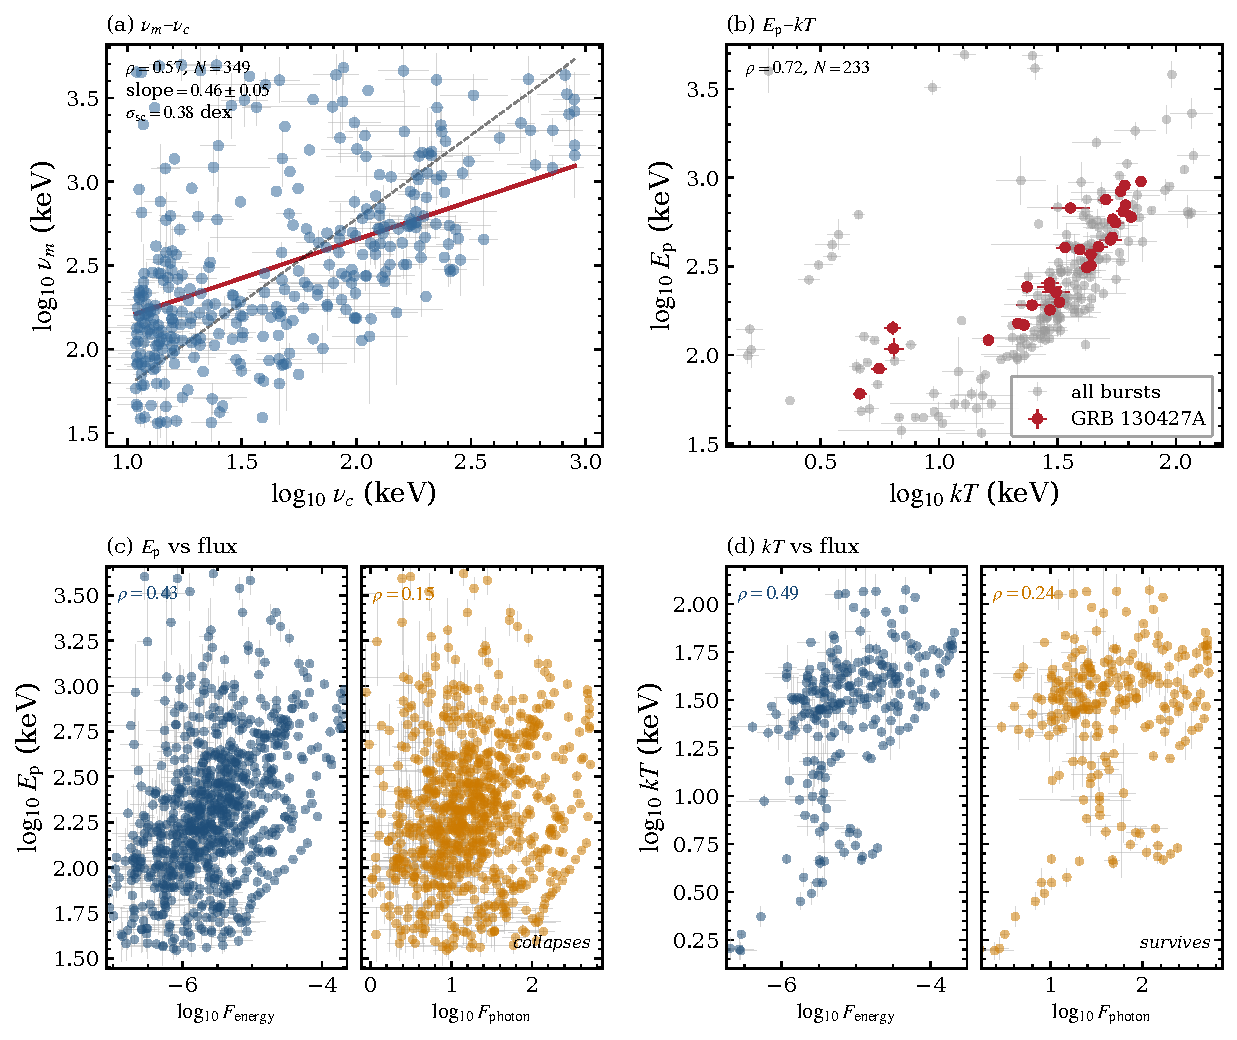
\includegraphics[width=0.92\textwidth]{two_break_figures/fig_corr.pdf}
\caption{Spectral-break and temperature correlations. (a) The two 2SBPL break
energies $\num$ vs $\nuc$ ($N=349$; red: \citealt{DAgostini2005}
errors-in-both-variables fit, slope $0.46\pm0.05$; dashed: 1:1). (b) The
$\Ep$--$\kT$ relation over the decisive-blackbody bins, with GRB~130427A
highlighted. (c) $\Ep$ vs energy flux (left, blue) and photon flux (right,
orange), sharing the $y$-axis: the correlation \emph{collapses} from
$\rho=0.43$ to $0.15$, showing it is largely induced by energy weighting.
(d) The same comparison for $\kT$: the correlation \emph{survives} in photon
flux ($\rho=0.24$; energy flux $0.49$), indicating a real thermal--intensity
link. Error bars are drawn where the fitted parameter is constrained
(relative uncertainty below 100\%; flux interval below 0.5~dex).}
\label{fig:corr}
\end{figure*}

% ============================================================================
\section{Assessment of Compatibility with Emission Models} \label{sec:emission}
% ============================================================================
\subsection{Spectral Shape} \label{sec:shape}
Optically-thin synchrotron limits the low-energy index to
$\alpha\le-2/3$ (slow cooling), steepening to $-3/2$ (fast cooling), whereas a
photosphere can be harder; a photospheric preference can be claimed with
confidence only for $\alpha>-0.5$ at high significance \citep{Acuner2020}. We
place the maximum $\alpha$ of each burst against \Ep\ and the synchrotron and
photospheric limiting lines (Figure~\ref{fig:lines}). We find that $74\%$
($74/100$) of bursts reach a peak $\alpha$ above the slow-cooling synchrotron line
($-2/3$) and $64\%$ ($64/100$) enter the photospheric region ($\alpha>-0.5$),
broadly consistent with the hard low-energy indices reported by \citet{Basak2014}
and \citet{Crider1997} and difficult to reconcile with pure fast-cooled
synchrotron.

\begin{figure}[t]
\centering
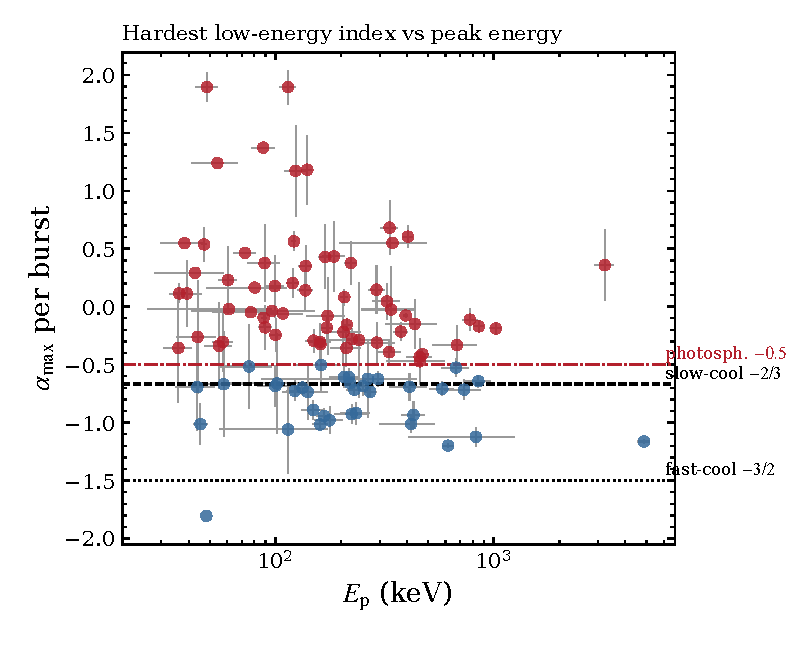
\includegraphics[width=\linewidth]{two_break_figures/fig_lines.pdf}
\caption{Hardest low-energy index per burst, $\alpha_{\rm max}$, vs \Ep, with the
slow- and fast-cooled synchrotron lines ($-2/3$, $-3/2$) and the photospheric
limit ($-0.5$). Red points (64/100) reach the photospheric region in at least one
bin. The few extreme values ($\alpha_{\rm max}\gtrsim1$) arise from weakly
constrained bins and carry correspondingly large uncertainties.}
\label{fig:lines}
\end{figure}

\subsection{Spectral Evolution and Correlations} \label{sec:evol-assess}
The curvature split (Section~\ref{sec:curv}) indicates that most single-pulse
curvature is statistically consistent with an added blackbody, with a minority
decisively requiring a second synchrotron break. The sub-dominant
$F_{\rm BB}/F_{\rm tot}$, the recovery of the $\Ep$--$\kT$ correlation only at
high signal-to-noise, and the survival of the $\kT$--intensity correlation in
photon flux ($\rho=0.24$, against $0.49$ in energy flux, where the
$\Ep$--intensity correlation collapses instead) together indicate that the
empirical continuum can mask a sub-dominant thermal component
\citep[cf.][]{Basak2014,Burgess2014b}.

% ============================================================================
\section{Discussion} \label{sec:discussion}
% ============================================================================
\subsection{Comparison with Previous Works on Single-Pulse GRBs}
\label{sec:disc-compare}
Single-pulse bursts have long been the preferred laboratory for prompt-emission
spectroscopy, and our sample of $106$ bursts is, to our knowledge, the largest
uniformly-analyzed set to date. Table~\ref{tab:compare} summarizes the
comparison; we discuss it thematically.

\emph{The single-pulse lineage and spectral evolution.}
\citet{Ryde2004} and \citet{RydePeer2009} established that a single FRED-like
pulse exhibits the simplest spectral evolution and is well described by a
blackbody-plus-power-law, making single pulses the cleanest test of the prompt
mechanism. \citet{Lu2012} classified the \Ep\ evolution of bright single-pulse
Fermi bursts into hard-to-soft (HTS) and intensity-tracking (IT) patterns, a
scheme extended by \citet{Basak2013,Basak2014}. Our rise-phase classification
(HTS $63\%$, IT $25\%$; Section~\ref{sec:evol}) recovers the same two modes and
the same HTS-dominated balance as those small samples. The agreement on the
low-energy index is also notable: our median Band $\alpha=-0.71$ matches the IT
mean ($-0.68$) of \citet{Basak2014} and is close to the slow-cooled value
$-0.81\pm0.1$ of \citet{Burgess2014b}. On the synchrotron line of death the
comparison must be made carefully: \citet{Basak2014} report $\alpha>-2/3$ in
$63.4\%$ of their HTS \emph{bins} ($74.6\%$ excluding GRB~110721A), whereas our
like-for-like per-bin fraction is $44\%$ over a sample dominated by IT-era
decay bins, and $74\%$ ($74/100$) of our \emph{bursts} exceed the line in at
least one bin. The numbers are therefore comparable rather than identical, but
all the single-pulse studies---including \citet{Basak2013} and
\citet{Guiriec2010}---find the line of death frequently violated, which we now
establish at population scale.

\emph{The thermal / multi-component program.}
A sub-dominant photosphere has been advocated through blackbody composites
\citep{Ryde2004,Guiriec2010,Guiriec2011,Guiriec2015,Basak2014}. \citet{Basak2014}
find that a blackbody-plus-power-law peaks at $\sim3kT$, below the Band $\nu
F_\nu$ peak, and favor multi-blackbody models over Band; \citet{Guiriec2015}
require a cutoff-power-law$+$blackbody$+$power-law for two bright GRBs, with the
blackbody carrying only $1$--$10\%$ of the energy ($kT\sim40$~keV) and argue that
the hard $\alpha$ values are an artifact of fitting Band to a multi-component
spectrum. Our results support this picture at scale: the thermal flux fraction
is sub-dominant (median $0.006$ with interquartile range $0.001$--$0.10$, the
upper quartile matching their $1$--$10\%$ energy range), our decisive blackbody
temperatures ($\kT\approx3$--$70$~keV, median $28$) bracket their
$\sim$$40$~keV, and $91\%$ ($151/166$) of curvature-requiring bins are equally
or better described by adding a sub-dominant blackbody than by a second
synchrotron break.

\emph{The synchrotron / physical-model program.}
\citet{Burgess2014a} fit a physical synchrotron$+$blackbody model to six
single-pulse bursts and reported a strong thermal--non-thermal correlation
($\Ep\propto\kT^{\alpha}$, pooled $\rho\approx0.8$, $\alpha\sim1$--$2$); we test
this at $\sim$$18\times$ the sample size and recover it in $89\%$ ($17/19$) of
the bursts with enough decisive-blackbody bins to test, most cleanly in the
highest-S/N bursts (GRB~130427A: $\rho=0.93$, slope $0.88\pm0.07$), consistent
with empirical continua absorbing the thermal curvature in fainter bursts. The
double-break synchrotron picture \citep{Oganesyan2017,Ravasio2018,Ravasio2019}
predicts the 2SBPL we fit; in the brightest GRB ever, GRB~221009A,
\citet{Ravasio2023} find a genuine second low-energy break only in the
highest-S/N intervals---directly mirroring our result that an explicit second
break wins decisively in just $9\%$ ($15/166$) of curvature bins (a lower
limit), epitomized by GRB~110721A. This is expected: \citet{Ravasio2018} showed
that the $+$BB and two-break descriptions separate only in bright spectra with
a large peak-to-break ratio ($E_{\rm peak}/E_{\rm break}\gtrsim10$), precisely
the high-S/N regime. Finally, \citet{Mei2025} find that the
synchrotron model is acceptable for most bursts, that they lie in a
fast/intermediate-cooling regime ($\num\gtrsim\nuc$), and that the
spectral--energetics link is $\nuc$--$\Liso$ rather than the Yonetoku relation. We
independently support the absence of an $\Ep$--luminosity relation: the apparent
$\Ep$--intensity correlation (energy-flux $\rho=0.43$) collapses in photon flux
($\rho=0.15$), while the $\kT$--intensity correlation survives ($\rho=0.24$); and
our 2SBPL bins, with $\nuc<\num$ by construction, sit in the same
marginally-fast-cooling regime.

\emph{Large catalogs and the degeneracy lesson.}
Compared with the broad GBM catalogs \citep{Kaneko2006,Gruber2014,Yu2016} and the
short-GRB Bayesian catalog of \citet{Burgess2019}---in which $513/525$ short-burst
spectra prefer a cutoff power law with no thermal component---our six-model
analysis adds an explicit thermal-versus-two-break decomposition. Our central
caution echoes \citet{Basak2014}: no single empirical model is decisively
preferred over the next-best alternative in $92\%$ ($875/950$) of comparable
bins, so distinguishing the emission mechanism requires physical models
\citep{Burgess2014b} or higher signal-to-noise, not empirical goodness-of-fit
alone. Throughout, we verify our main results on the cleanest (Gold) subsample.

\subsection{The Two-Break Relation} \label{sec:disc-breaks}
The pooled $\num$--$\nuc$ correlation ($\rho=0.57$, $N=349$) is present both
between bursts ($\rho=0.51$) and within bursts: beyond the pooled
mean-subtracted residuals ($\rho=0.43$), the cluster-honest per-burst test
gives a median per-burst $\rho=0.50$, positive in $41/54$ bursts with
$\ge$$3$ double-break bins (sign-test $p=2\times10^{-4}$). The relation is
therefore not merely an inter-burst trend: harder bursts have both breaks at
higher energies, and within a burst the two breaks move together. Its slope,
however, depends on the estimator because the intrinsic scatter is large: the
\citet{DAgostini2005} fit gives $0.46\pm0.05$ (\ssc$=0.38$~dex), restricting to
bins with both breaks constrained gives $0.64\pm0.05$ ($\rho=0.67$, $N=253$),
and symmetric unweighted regression gives $1.05\pm0.06$; we therefore regard
the \emph{existence} of the correlation, not its slope, as the robust result.
It is also robust to the fit boundary: excluding the $26\%$ of \nuc\ values
within a factor of two of the 8~keV NaI edge leaves $\rho=0.55$ ($N=260$).
Because \nuc\ and \num\ are breaks of the same spectrum fit simultaneously,
part of the within-burst correlation can be induced by their joint estimation;
we note, however, that time-resolved \emph{physical} synchrotron fits of
GRB~180720B show the cooling and injection energies decreasing together
through the burst with $E_{\rm m}/E_{\rm c}\approx13$--$22$
\citep{Ronchi2020}---the same co-evolution, recovered with a model in which
the two breaks are not independently adjustable shape parameters. The
physically meaningful quantity is the ratio $\num/\nuc$ (the cooling
regime). Since the 2SBPL fit enforces $\nuc<\num$, the bins with a measurable
double break sit in the fast-cooling regime by construction; quantitatively,
the ratio distribution has a median $\num/\nuc\simeq6$ (interquartile
$3$--$13$), with $21\%$ ($75/349$) in the intermediate regime
$1<\num/\nuc<3$ of \citet{Mei2025}---close to the $\sim$$25\%$ they find in
their time-resolved sample, and well below the $\sim$$60\%$ of their
single-peak-bin sample. \citet{Mei2025} use this ratio as a cooling-regime
classifier rather than fitting a break--break relation; within the single burst GRB~160625B,
\citet{Ravasio2018} found $E_{\rm peak}$--$E_{\rm break}$ positively correlated
($\rho=0.61$), consistent in sign with our within-burst result. Our positive
$\num$--$\nuc$ correlation is, to our knowledge, the first such relation
reported for a large single-pulse \emph{sample}, and warrants confirmation
with physical synchrotron fits.

\subsection{Implication for the Radiation Process} \label{sec:disc-radiation}
The low-energy index peaking near $\alpha\approx-0.7$, between the
synchrotron limits but with a substantial fraction of bursts above them, is
consistent with marginally-fast/slow-cooled synchrotron with ongoing
acceleration in some bursts and a photospheric contribution in others
\citep[cf.][]{Basak2014,Burgess2014b}. Mapping the $\Ep$--$\kT$ slope to the
outflow via $\Gamma\propto r^{\mu}$ \citep{Burgess2014a}, $\alpha\!\sim\!1$
indicates a baryon-dominated and $\alpha\!\sim\!2$ a magnetically-dominated
jet; the slope we recover for the cleanest case, GRB~130427A
($\Ep\propto\kT^{0.88\pm0.07}$, \citealt{DAgostini2005} fit), is consistent
with the baryon-dominated value, but we stress that with empirical (not
physical) models this mapping is only indicative. The clearest two-break burst
in our sample, GRB~110721A (2SBPL-preferred, $F_{\rm BB}/F_{\rm
tot}\approx0.001$), is the counter-example in which the curvature is genuinely
a second synchrotron break rather than a thermal component.

% ============================================================================
\section{Summary} \label{sec:summary}
% ============================================================================
In this paper, we performed time-resolved empirical spectroscopy of $106$
single-pulse, bright Fermi/GBM bursts ($1057$ spectra; six models each), one
of the largest uniform single-pulse spectral surveys to date. Our main findings
are as follows.
\begin{enumerate}
\item The low-energy index peaks at $\alpha\approx-0.7$, near the slow-cooled
  synchrotron limit, with $74\%$ ($74/100$) of bursts reaching harder values in
  at least one bin; the rise-phase \Ep\ evolution is HTS-dominated
  ($63\%$, $48/76$), as in previous single-pulse samples.
\item Of the bins requiring curvature beyond a single break, $91\%$ ($151/166$)
  are equally or better described by adding a blackbody than by an explicit
  second break (the $9\%$ two-break fraction is a lower limit); no single model
  is decisively preferred over the next-best in $92\%$ ($875/950$) of
  comparable bins.
\item The \citet{Burgess2014a} $\Ep$--$\kT$ correlation is recovered in $89\%$
  ($17/19$) of the bursts with enough decisive-blackbody bins to test
  (GRB~130427A: $\rho=0.93$, $\Ep\propto\kT^{0.88\pm0.07}$), but fainter bursts
  cannot be tested with empirical models---a model-sensitivity, not a sample,
  limit.
\item The two 2SBPL break energies are positively correlated ($\rho=0.57$;
  \citealt{DAgostini2005} slope $0.46\pm0.05$, \ssc$=0.38$~dex), both within
  and between bursts.
\end{enumerate}
We conclude that the dominant spectral curvature of bright single-pulse GRBs is
more economically described by a sub-dominant photospheric component than by a
second synchrotron break, with a genuine two-break minority---epitomized by
GRB~110721A---in which the cooling and injection frequencies are correlated.

\begin{acknowledgments}
% %TODO grants, data acknowledgments.
This work made use of \textsf{3ML} \citep{Vianello2015} and the Fermi/GBM and LAT
public data; Bayesian blocks follow \citet{Scargle2013} and correlation fits the
\citet{DAgostini2005} method.
\end{acknowledgments}
\facilities{Fermi(GBM), Fermi(LAT)}
\software{3ML \citep{Vianello2015}, Astropy, Matplotlib, NumPy, SciPy, emcee
\citep{ForemanMackey2013}}

% ---- Tables (Li-style; representative rows + machine-readable full versions) ----
\begin{deluxetable}{lccccc}
\tablecaption{Global properties of the sample (representative rows).\label{tab:sample}}
\tablehead{\colhead{GRB} & \colhead{$T_{90}$ (s)} & \colhead{Fluence} &
\colhead{NaI} & \colhead{LAT} & \colhead{$N_{\rm bins}$}}
\startdata
130427A & 138.2 & $2.5\times10^{-3}$ & n6 & Y & 65 \\
160625B & 453.4 & $6.4\times10^{-4}$ & n6 & Y & 57 \\
150902A & 13.6  & $8.3\times10^{-5}$ & n0 & Y & 19 \\
110721A & 21.8  & $3.7\times10^{-5}$ & n6 & Y & 11 \\
081125A & 9.3   & $1.9\times10^{-5}$ & na & N & 8  \\
\enddata
\tablecomments{Fluence in erg~cm$^{-2}$ (10--1000~keV, GBM catalog). The full
machine-readable table lists all $106$ bursts; selection is on pulse shape, not
duration.}
\end{deluxetable}

\begin{deluxetable}{lcccc}
\tablecaption{Block grading and preferred model (representative rows).\label{tab:perburst}}
\tablehead{\colhead{GRB} & \colhead{$N$ bins} & \colhead{Grade} &
\colhead{Preferred model} & \colhead{$F_{\rm BB}/F_{\rm tot}$}}
\startdata
130427A & 65 & Gold   & Band$+$BB & 0.12  \\
160625B & 57 & Gold   & Band$+$BB & 0.004 \\
150902A & 19 & Gold   & Band$+$BB & 0.13  \\
110721A & 11 & Gold   & 2SBPL     & 0.001 \\
081125A & 8  & Silver & Band$+$BB$^{\rm a}$ & 0.002 \\
\enddata
\tablecomments{Preferred model is the most frequent physically valid AIC winner
across a burst's bins ($^{\rm a}$tied with Band); $F_{\rm BB}/F_{\rm tot}$ is
the per-burst median over decisive-blackbody ($\daic\ge10$) bins. The full
per-burst table and the complete per-bin fit catalog ($1057$ rows: times,
parameters with uncertainties, information criteria, and likelihood-ratio
statistics for all six models) are available in machine-readable form.}
\end{deluxetable}

\begin{deluxetable}{lcccc}
\tablecaption{Band-parameter means $\pm$ standard deviation per tier.\label{tab:dist}}
\tablehead{\colhead{Tier} & \colhead{$N_{\rm GRB}$} & \colhead{$N_{\rm spec}$} &
\colhead{$\langle\alpha\rangle$} & \colhead{$\langle\log_{10}\Ep\rangle$}}
\startdata
Gold   & 40 & 521 & $-0.71\pm0.43$ & $2.34\pm0.41$ \\
Silver & 44 & 226 & $-0.52\pm0.58$ & $2.28\pm0.38$ \\
Bronze & 22 & 45  & $-0.66\pm0.51$ & $2.27\pm0.38$ \\
\enddata
\tablecomments{Pooled blackbody temperature over the $301$ decisive-blackbody
bins ($\daic\ge10$): median $\kT=28.5$~keV (5--95\%: $3.4$--$70$~keV).}
\end{deluxetable}

\begin{deluxetable}{lcccc}
\tablecaption{K-S comparison of tier distributions (Gold vs.\ Silver$+$Bronze).\label{tab:ks}}
\tablehead{\colhead{} & \multicolumn{2}{c}{$\alpha$} & \multicolumn{2}{c}{$\log_{10}\Ep$}}
\startdata
        & $D$  & $p$    & $D$  & $p$    \\
Gold vs.\ rest & 0.13 & 0.004 & 0.11 & 0.031 \\
\enddata
\end{deluxetable}

\begin{deluxetable*}{lccccc}
\tablecaption{Pooled correlation results across all valid time bins.\label{tab:curv}}
\tablehead{\colhead{Relation ($y$ vs $x$)} & \colhead{$N$} & \colhead{$\rho$} &
\colhead{$p$} & \colhead{slope} & \colhead{\ssc\ (dex)}}
\startdata
$F$ vs $\alpha$        & 792 & $0.17$ & $3\times10^{-6}$  & $k=0.27$        & $0.65$ \\
$F$ vs $\Ep$           & 792 & $0.43$ & $<10^{-36}$       & $0.66$          & $0.59$ \\
$\alpha$ vs $\Ep$      & 792 & $0.10$ & $3\times10^{-3}$  & $0.02$          & $0.49^{\dagger}$ \\
$\Ep$ vs $\kT$         & 233 & $0.72$ & $3\times10^{-38}$ & $0.56$          & $0.36$ \\
$\num$ vs $\nuc$       & 349 & $0.57$ & $<10^{-30}$       & $0.46\pm0.05$   & $0.38$ \\
$\kT$ vs flux          & 233 & $0.24$ & $2\times10^{-4}$  & $0.18$          & $0.36$ \\
\enddata
\tablecomments{$\rho$ is the Spearman coefficient. Slopes are least-squares
log--log fits ($k$ is the e-folding index of $F=F_0e^{k\alpha}$); \ssc\ is the
residual rms in dex, except $^{\dagger}$ which is in units of $\alpha$. The
$\num$--$\nuc$ slope and \ssc\ are the \citet{DAgostini2005}
errors-in-both-variables values with free intrinsic scatter (unweighted
orthogonal regression gives $1.05\pm0.06$; least-squares $0.56$). $\kT$ rows
use the decisive-blackbody bins with valid Band flux. Energy fluxes are
observer-frame (no redshifts). $F$--$\Ep$ uses energy flux and is partly
induced (photon-flux $\rho=0.15$); $\kT$--flux uses photon flux (energy-flux
$\rho=0.49$). The $\num$--$\nuc$ relation holds within bursts ($\rho=0.43$
pooled; median per-burst $\rho=0.50$) and between bursts ($\rho=0.51$).}
\end{deluxetable*}

\begin{table*}
\centering
\caption{Comparison with previous single-pulse / prompt-emission spectral
studies.\label{tab:compare}}
\footnotesize
\newcommand{\kf}[1]{\parbox[t]{7.2cm}{\raggedright #1\strut}}
\begin{tabular}{llll}
\hline\hline
Study & Sample & Models & Key finding and relation to this work \\
\hline
\citet{RydePeer2009} & BATSE single pulses & BBPL & \kf{Photospheric BBPL; single pulses as the cleanest laboratory (rationale we adopt).} \\
\citet{Lu2012} & $51{+}11$ GBM & Band & \kf{HTS/IT \Ep-evolution classes; we recover both, HTS-dominated (HTS $63\%$/IT $25\%$).} \\
\citet{Basak2013} & 19 GRB/43 pulses & Band & \kf{Pulse-wise Amati; $\alpha$ sometimes $>-2/3$.} \\
\citet{Basak2014} & 9 single-pulse & BBPL/mBBPL/2BBPL & \kf{BB peaks $\sim3kT$ below the Band peak; $\alpha>-2/3$ in $63.4\%$ of HTS bins; favor multi-BB. Comparable to our per-bin $44\%$ / per-burst $74\%$, at $\sim$$12\times$ the scale.} \\
\citet{Burgess2014a} & 6 single-pulse & synch.$+$BB & \kf{$\Ep$--$\kT$ correlation ($\rho\approx0.8$); we recover it in $17/19$ testable bursts (130427A $\rho=0.93$).} \\
\citet{Burgess2014b} & 8 single-pulse & physical synch. & \kf{Slow-cooled $\alpha=-0.81$; BB in $5/8$; fast cooling excluded.} \\
\citet{Guiriec2015} & 2 bright & C$+$BB$+$PL & \kf{Sub-dominant BB ($1$--$10\%$ energy, $kT\sim40$ keV); hard $\alpha$ a Band-fit artifact. Our decisive-BB bins: $F_{\rm BB}/F_{\rm tot}$ up to $\sim$$0.1$, $kT\approx3$--$70$ keV.} \\
\citet{Ravasio2023} & GRB 221009A & SBPL/2SBPL & \kf{Genuine 2nd break only at highest S/N; mirrors our $9\%$ two-break lower limit (e.g.\ 110721A).} \\
\citet{Mei2025} & $74$ single-bin $+\,13$ t.r. & physical synch. & \kf{Fast/intermediate cooling; $\nuc$--$\Liso$, no Yonetoku. We confirm $\Ep$--flux is induced.} \\
\citet{Burgess2019} & 321 short & Band/CPL & \kf{Short bursts CPL-dominated ($513/525$); no thermal component.} \\
\textbf{This work} & \textbf{106 single-pulse} & \textbf{6 empirical} & \kf{\textbf{$91\%$ thermal-or-degenerate vs $9\%$ 2nd break (lower limit); $92\%$ (875/950) without a decisive winner; $\num$--$\nuc$ correlated.}} \\
\hline
\end{tabular}
\\[3pt]
{\footnotesize \textbf{Notes.} ``t.r.''~$=$~time-resolved; all samples are
Fermi/GBM ($\pm$LAT) unless noted. This work extends the single-pulse approach to
the largest uniform sample.}
\end{table*}

\appendix
\section{Fit Configuration} \label{app:fitconfig}
All fits use MINUIT within 3ML, each time bin seeded from the burst's
time-integrated fit. Table~\ref{tab:fitconfig} lists the free parameters,
allowed ranges, and default seeds for each model component. Cross-detector
effective-area constants are free within $0.8$--$1.2$ (frozen to unity for the
reference NaI). The blackbody multi-start re-fits each $+$BB model whose
blackbody is railed or insignificant from three seeds (component defaults with
$\kT=30$~keV; the time-integrated seed with $\kT=30$ and with $80$~keV),
retaining the lowest $-2\ln L$. The physical-validity gate declares a fit
non-physical when any key shape parameter lies within $0.1\%$ of its allowed
span from a bound, or when the 2SBPL breaks are mis-ordered ($x_b\ge x_p$);
non-physical fits remain in the catalog but cannot be selected as the
preferred model, and in $4\%$ ($43/1057$) of bins no model passes the gate and
no preferred model is assigned. The complete per-bin fit catalog ($1057$ rows)
and the full per-burst sample table are available as machine-readable tables.

\begin{deluxetable}{llll}
\tablecaption{Free parameters, allowed ranges, and seeds.\label{tab:fitconfig}}
\tablehead{\colhead{Model} & \colhead{Parameter} & \colhead{Range} & \colhead{Seed}}
\startdata
Band   & $\alpha$        & $(-1.9,\,1.9)$   & $-1.0$ \\
       & \Ep\ (keV)      & $(30,\,5000)$    & $200$  \\
       & $\beta$         & $(-5,\,-1.6)$    & $-2.25$ \\
CPL    & $\Gamma$        & $(-2,\,1)$       & $-1.0$ \\
       & $E_c$ (keV)     & $(10,\,5\times10^4)$ & $200$ \\
SBPL   & $\alpha$        & $(-2.5,\,1.5)$   & $-1.0$ \\
       & $E_{\rm b}$ (keV) & $(10,\,5000)$  & $300$  \\
       & $\beta$         & $(-5,\,-1.5)$    & $-2.25$ \\
2SBPL  & $\alpha_1$      & $(-2.5,\,2.5)$   & $-0.66$ \\
       & $x_b$ (keV)     & $(10,\,900)$     & $50$   \\
       & $\alpha_2$      & $(-3,\,0.5)$     & $-1.5$ \\
       & $x_p$ (keV)     & $(30,\,5000)$    & $200$  \\
       & $\beta$         & $(-5,\,-1.5)$    & $-2.25$ \\
BB     & \kT\ (keV)      & $(1,\,200)$      & $30$   \\
\enddata
\tablecomments{Normalizations are free with broad ranges. SBPL break scale and
2SBPL sharpnesses ($n_1=n_2=2$) are held fixed in this run
(Section~\ref{sec:models}). The $x_b$ upper bound reflects the NaI band.}
\end{deluxetable}

% ============================================================================
% Author-year natbib: every \bibitem optional arg MUST contain (YYYY).
% %chk cross-check all volume/page numbers against ADS before submission.
% ============================================================================
\bibliographystyle{aasjournal}
\bibliography{two_break}


\end{document}
